\startchapter{Real-time Cutting}
\label{chapter:Cutting}
The physics simulation in our system uses tetrahedral meshes to compute deformations.
One of the main objectives of virtual reality based surgical simulation systems is the removal of pathologic tissue 
\cite{Steinemann, Nienhuys2001a}. Cutting imposes many challenges in the development of a robust, interactive surgery 
simulation, not only because of the nonlinear material behavior exhibited by soft tissue but also due to the
complexity of introducing the cutting-induced discontinuity. In most publications, the progressive surgical cutting is modelled
by the conventional finite element (FE) method, in which the high computational cost and error accumulation due to re-meshing constrain 
the computational efficiency and accuracy \cite{Steinemann, Courtecuisse2010a}. 

We developed our new cutting approach in the context of a human skull craniotomy simulation. When an abnormality of the brain is suspected, 
Stereo-tactic (probing in three dimensions) brain needle biopsy is performed and guided precisely by a computer system to avoid 
serious complications. A small hole is drilled into the skull, and a needle is inserted into the brain tissue guided by computer-assisted 
imaging techniques (CT or MRI scans). The actual biopsy process can not be seen by the surgeon. For this reason,
non-progressive cutting, where a tetrahedral element is decomposed after the sweep surface traverses the tetrahedral elements, is a reasonable
approximation for our application area, and so we define the cut once the instrument has traversed the tissue. 
Moreover, there is little, if at all, resistance to the cut tool movement through the tissue. Therefore, in the current stage, we do 
not model any haptic interaction of the cutting tool with the deformable object during a cut. 


\section{Related Work}
A number of approaches has been proposed by the computer graphics community to enable cutting of deformable models. 
Except for a few methods most of them use tetrahedral meshes for the volumetric mesh representation. 
Bielser \etal performed an adaptive refinement of the tetrahedral elements cut by a virtual scalpel \cite{Bielser1999}.

Mor \etal tried to reduce the number of sub-elements created while cutting tetrahedral meshes \cite{Mor2000}.
One of the major issues in cutting is the creation of ill-shaped elements i.e. skinny elements, which can adversely affect the
performance and stability of the system solver. Some works attempted to avoid such elements via mesh alignment techniques 
\cite{Nienhuys2001a, Steinemann2006}. Other methods tried to solve the issue by removing them completely.

Jin \etal proposed a meshless total Lagrangian adaptive dynamic relaxation cutting algorithm to predict the steady-state 
responses of soft tissue \cite{Jin2013}. A cloud of points is used for discretization and approximation of the deformation 
field within the continuum without generation of finite element meshes. They didn't report 
any performance measurements and the quality of the cuts could not be verified with the simple truth cube model they reported in their paper.
 
Wu \etal \cite{Wu2011} proposed an algorithm for 3D mesh cutting using a combination of the adaptive octree refinement with an iterative composite
element hierarchy to enable simulating high-resolution cuts with a small number of degrees of freedom (DOFs). 
They used the dual contouring method \cite{Ju2002} to keep the sharp creases along the cut. Due to the high computational cost and naive implementation 
their method is not scalable and has yet to become an interactive cutting approach.

In a closely related work Courtecuisse \etal presented a soft-tissue cutting system with haptic 
feedback \cite{Courtecuisse2010a}. Their cutting strategy follows Mor \etal  \cite{Mor2000} work and 
suffers from jagged lines along the cut surface as shown in their examples of a laparoscopic hepatecotomy.
The progressive cutting is not supported in their system and as most of the other works in this area they produce too many
new nodes when subdividing cut elements.

Jerabkova \etal proposed a solution to ill-shaped elements problem by using hexahedral elements instead of 
tetrahedra \cite{Jerabkova2010}. Their approach relies on fine-level voxels to model object surface and simulate cutting. 
The volume data requires more memory space than traditional, surface-based models. Cutting is performed by
removing voxels. For sufficiently small voxels this typically remains unnoticeable but it may result in 
significant volume loss in case of a large number of cuts. 


Sifakis \etal \cite{Sifakis2007} proposed a geometric algorithm for placing cracks and incisions on 
tetrahedralized deformable objects. Their method is similar to the virtual node algorithm in that they avoid 
sliver elements and their associated stringent timestep restrictions. Producing ill-conditioned triangles on 
the material surface can have a negative effect on collision handling specially in case of a self collision.
Also in their system a cut that partially intersects a tetrahedron without separating it into disconnected 
fragments will not allow the material to separate within that embedding tetrahedron.

Steinemann \etal \cite{Steinemann} created a hysteroscopy simulator and minimized the number of added elements 
after a tetrahedral subdivision by cutting along existing edges and faces. The problem with their system is that
the result of the cutting is produced only after it has been completed and this leads to a delay in the system. 
Unfortunately they didn't report any performance statistics of their algorithm. 

In the following sections we provide an overview of the system and the data structures involved in the process 
and our cutting algorithm. The chapter is concluded by the analysis of the simulation results.

\section{Overview}
We present a GPU-assisted approach to cutting tetrahedral meshes in real-time. 
The input to our system is a cut trajectory and an edge-based data structure representing the tetrahedral mesh. 
As shown in figure \ref{fig:sweepsurf}, the user moves the cutting tool and the system records the path of the 
blade endpoints shown in purple. The first intersection between the recorded trajectory and the model marks the 
beginning of the cutting process. When the tool completely traverses the model the system computes the cutting
configurations as described below. The following steps are performed to complete the cut induced by the scalpel on the mesh:

\begin{figure}[H]
  \centering
  % the following command controls the width of the embedded PS file
  % (relative to the width of the current column)
  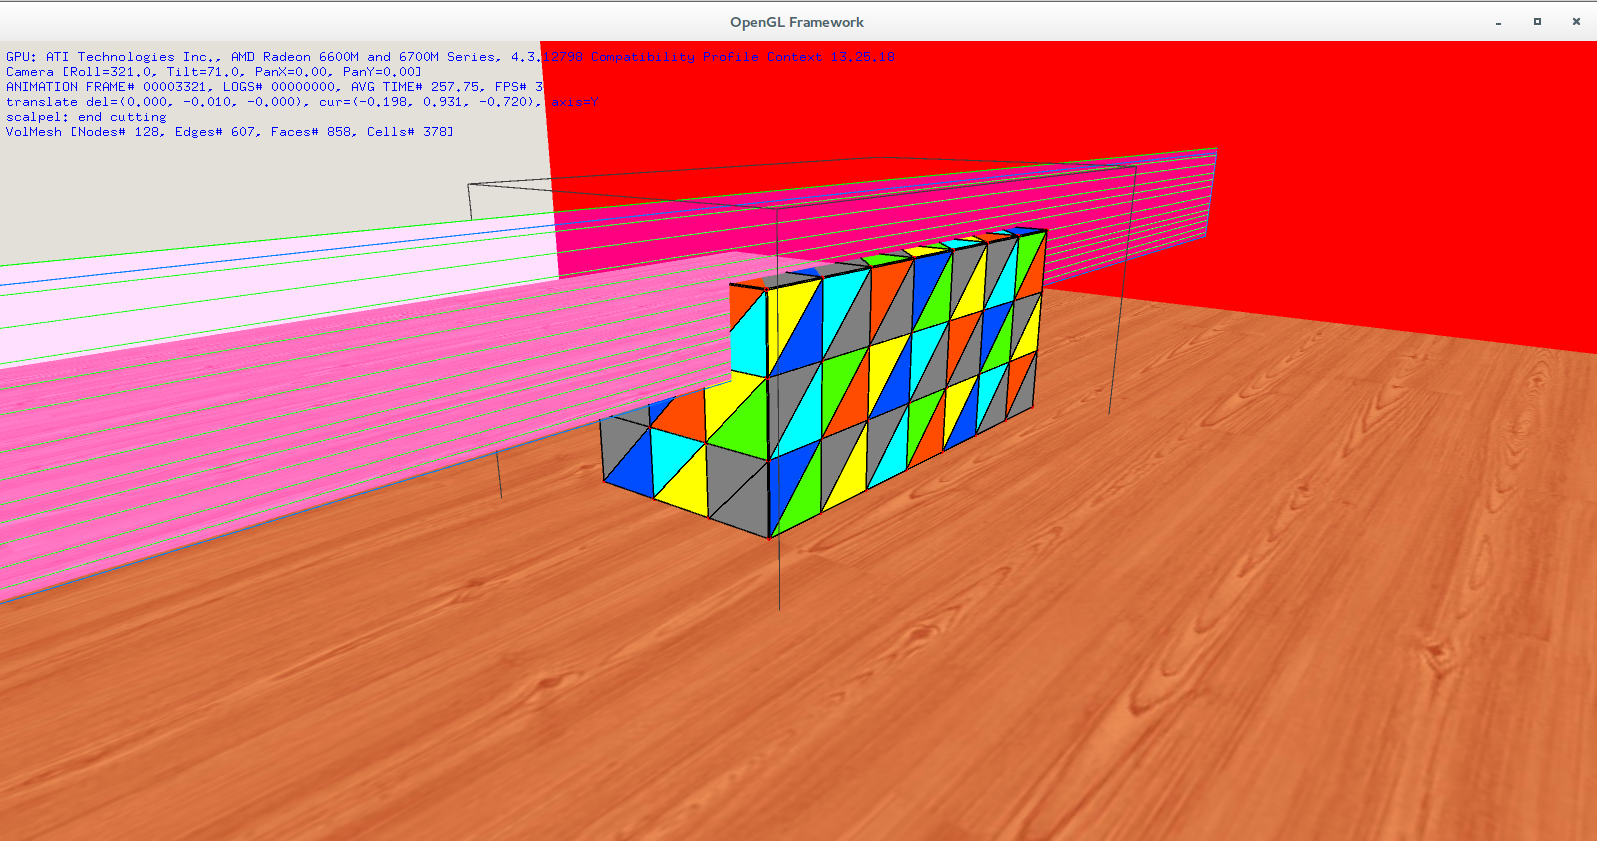
\includegraphics[width=0.6\linewidth]{figures/cutting/cubecut02.png}
  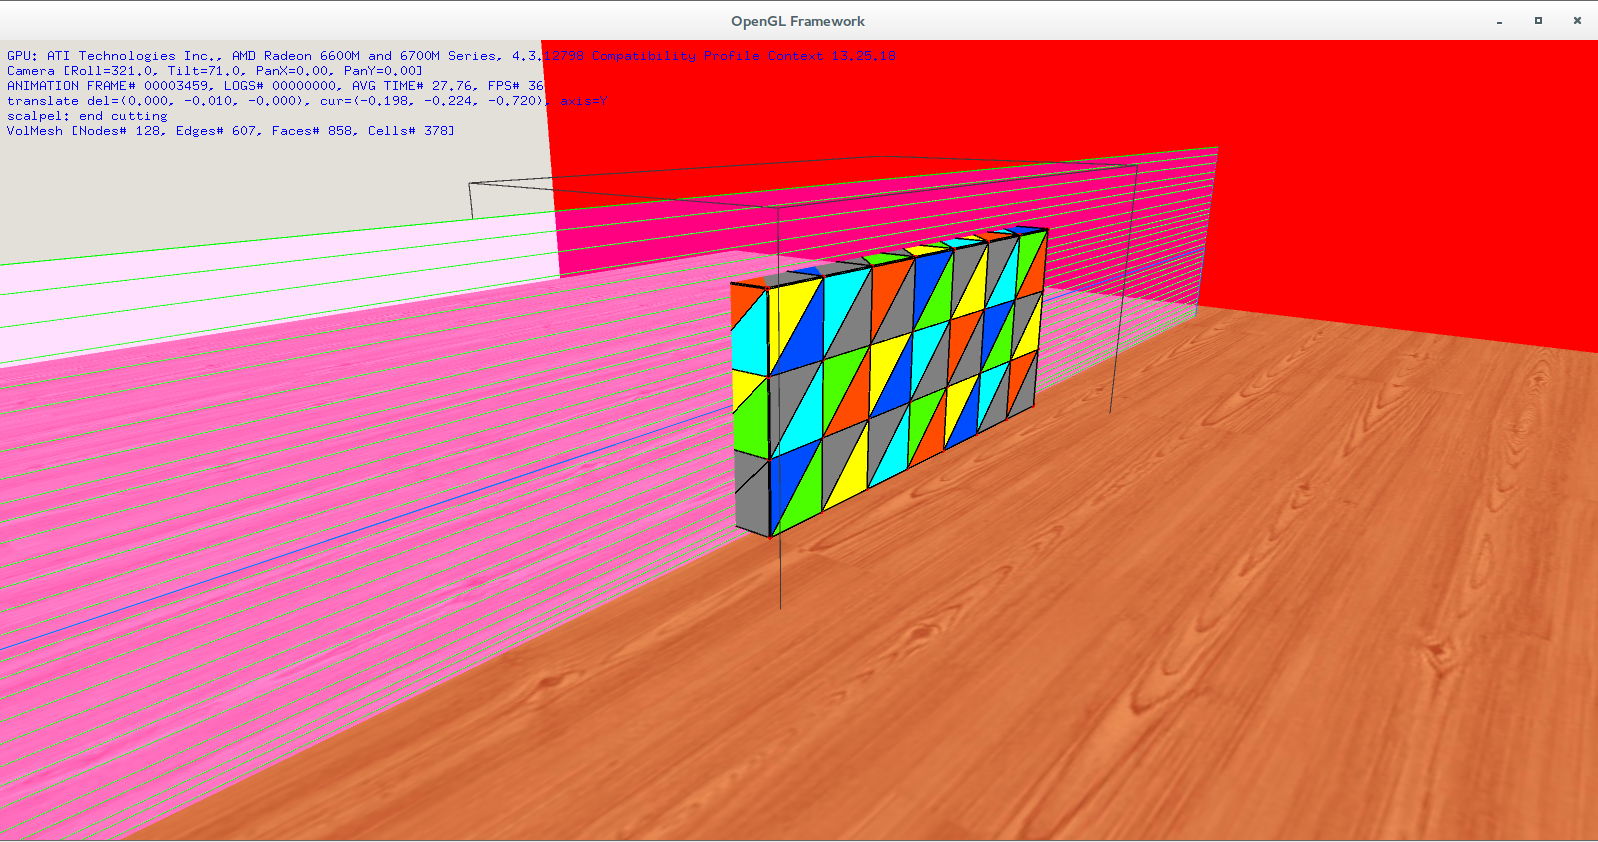
\includegraphics[width=0.6\linewidth]{figures/cutting/cubecut04.png}
  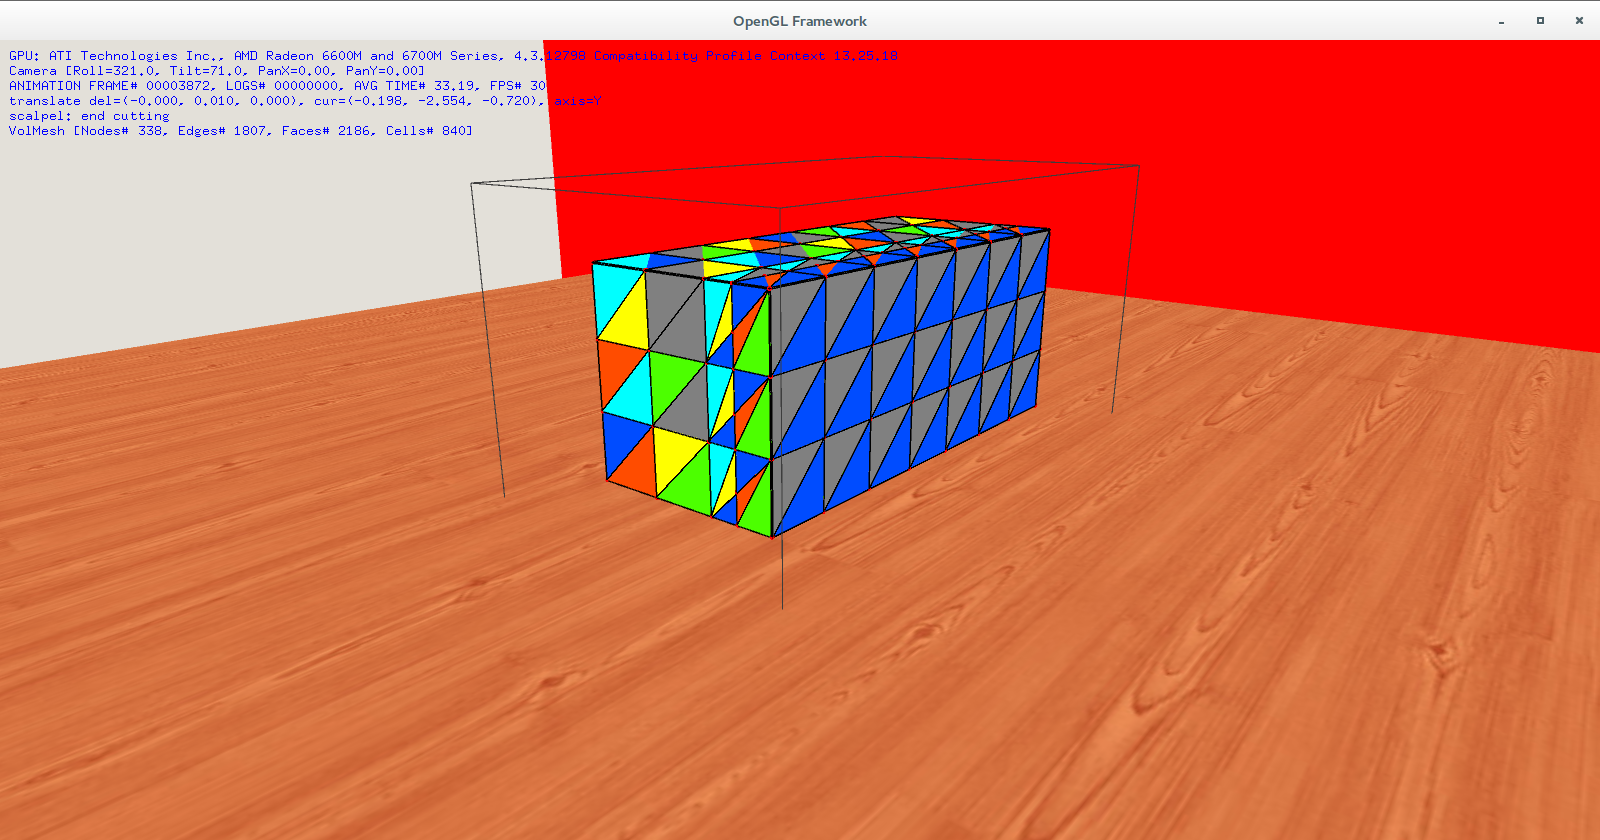
\includegraphics[width=0.6\linewidth]{figures/cutting/cubecut05.png}
  \caption{\label{fig:sweepsurf}
  {The cut trajectory in blue and the sweep-surface shown in pink. The scalpel passes through the voxel grid model for cutting.}
}
\end{figure}

\begin{enumerate}
 \item Using the GPU-accelerated algorithm the intersection of the sweep-surface and all the edges of the mesh 
 are computed. The output of this stage is a list of cut-edges and their associated intersection points. 
 
 \item A GPU kernel function is used to compute the distance of the nodes in the cut-edges and the end points of 
 the cut tool. This way the nodes that are too close to the sweep-surface are identified and a different configuration 
 is used to produce subdivided elements in the next stage to avoid ill-shaped elements. The output of this stage is 
 a list that associates edges with their cut-nodes.
 
 \item Using a look-up table all the cut tetrahedra are decomposed into sub-elements
 
 \item The nodes identified to be close enough to the cut trajectory are snapped to the sweep surface
 
 \item The solver system is synchronized with the latest mesh changes, all the mass, damping and stiffness 
 matrices are updated.
\end{enumerate}


\section{Data structure}
The tetrahedron is the three-dimensional case of the more general concept of a Euclidean simplex. 
Figure \ref{fig:tetconfig3} shows the structure of a tetrahedral element and the order we chose to 
name the nodes, edges and faces in its canonical orientation. In this figure $P_0$ to $P_3$ are
the nodes (i.e. degrees of freedom in the context of system deformation computation), $e_0$ to $e_5$ the edges 
and $F_0$ to $F_3$ are the faces of the element.

\begin{figure}[H]
  \centering
  % the following command controls the width of the embedded PS file
  % (relative to the width of the current column)
  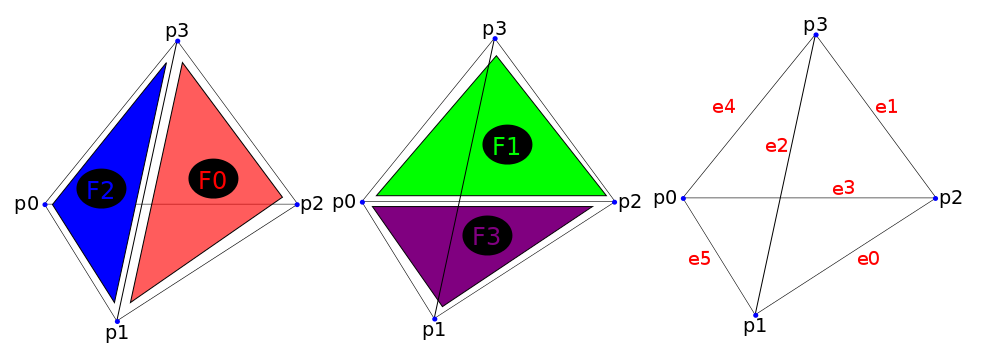
\includegraphics[width=1.0\linewidth]{figures/cutting/tetconfig3.png}
  \caption{\label{fig:tetconfig3}
  {A tetrahedral element in its canonical view. Iterating over nodes, edges and faces of each element is
  one of the primary operations in a geometric algorithm that manipulates such elements. The order we chose here is not the
  only possible one but it simplifies the cutting algorithm and element subdivision process as we will see later.}
}
\end{figure}


In a complex mesh of tetrahedral elements accessing each of these components is a necessary requirement for 
implementing any topological modifications. Therefore the main module in our cutting algorithm is an edge-based
data structure that maps tetrahedral elements to their associated faces and the faces to their associated edges and
finally the edges to their nodes. 

The minimal set of operations frequently used by most algorithms are as following \cite{Mario2010PolygonMesh}:

\begin{itemize}
 \item Access to individual vertices, edges, faces and tetrahedral elements. This includes the enumeration of 
 all elements in unspecified order.
 
 \item Per each vertex, access to all the directly adjacent nodes to that vertex (i.e. one ring neighborhood see figure \ref{fig:meshlinks}). 
 A typical use-case for this operation is the uniform distribution of the external forces applied to the mesh. 
 Also many mesh simplification algorithms are based on such operators.
 
 \item Top-down and bottom-up hierarchical access to the mesh entities (An example is shown in figure \ref{fig:meshlinks}). Top-down access 
 is inherently provided in the structure of the mesh entities e.g. elements are comprised of faces and faces are made up of set of edges etc. 
 In case of the bottom up access some algorithms will benefit to have the incident edges of a certain node, or in case of edges all the incident 
 faces of a given edge and for a given face all the incident elements to a particular face in the mesh. This type of access patterns are particularly 
 useful for topological modification scenarios and the required book-keeping operations.
 
 \begin{figure}[H]
  \centering
  % the following command controls the width of the embedded PS file
  % (relative to the width of the current column)
  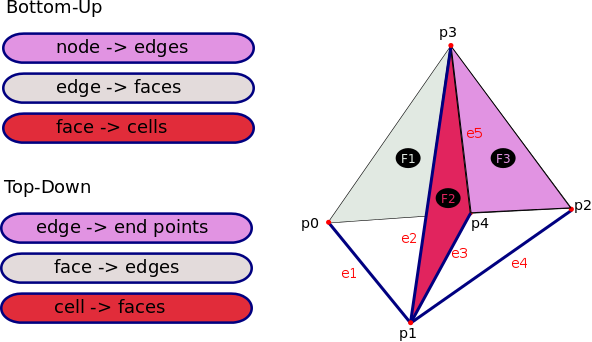
\includegraphics[width=0.8\linewidth]{figures/cutting/mesh_links.png}
  \caption{\label{fig:meshlinks}
  {Top-down and bottom-up mesh links. The top-down relationships is explicitly defined in the structure of the mesh.
  An example of the bottom-up links is shown here: Edges $e_1..e_4$ are incident to node $p_1$ and therefore the set 
  $\{p_0$, $p_2$, $p_3$, $p_4\}$} is the one-ring neighborhood of node $p_1$. Faces $F_1..F_3$ are incident to edge 
  $e_5$ and both tetrahedral cells are incident to face $F_2$.
}
\end{figure}

 \item Insertion and removal operations for nodes, edges, faces and elements. These operations require extra care in order to keep
 the top-down and bottom-up links up-to-date. As we will see in our cutting algorithm deferred removal operations can make matters alot simpler by
 delaying the actual removal until after all the identified entities are being visited and the new entities inserted to the structure.
 This is due to the fact that removal operations will update the internal links between mesh entities therefore two consecutive access operations
 might find the mesh at different states which is not intended in the original proposed algorithm.
 
 \item Update operations for nodes, edges, faces and elements. What is important here is to keep the top-down and bottom-up links up-to-date. 
 For-instance in case of an edge update as soon as the two endpoints of the edge is modified all the incident faces (higher level entity) 
 of that edge and also all the incident edges of the end points of the edge (lower level entity) should be updated.
\end{itemize}

The rest position of each node is stored which can be used to update the physics model and to interpolate the position 
of newly added nodes in case of cutting. Accessing edges using the bottom-up structure is expensive: First the list of incident 
edges to one of the endpoints of the edge is accessed and then a serial search on that list is done to find an edge with the matching 
end points. This has logarithmic complexity with respect to the number of edges in the structure. Instead we chose to use a hash-table
to access edges using a key derived from the two end-points of the edge. Below is how this key is computed for a given edge 
\cite{Mario2010PolygonMesh, Bloomenthal1997}:

\begin{equation}
 key64 = (nodes\left[ 1 \right] << 32) \And nodes\left[ 0 \right]
\end{equation}

This computation is performed when a new edge in inserted into the structure and can produce keys for $2^{64}$ edges uniquely. 
The hash-map then associates this key to its corresponding edge index thereby providing constant-time access. 
Using this technique the faces can also be accessed though their associated node indices which can be convenient for some applications. 

Nothing is removed directly from the our mesh storage buffers but rather upon cutting, the elements
are added to the $freelist$ and later the garbage collection removes all the $freelist$ items from the mesh storage buffers. 

When cutting an edge, an edge-update process is performed followed by a new edge insertion. 
The update process splits the original edge in two. Algorithm \ref{alg:edgesplit} describes this process (also see figure \ref{fig:splitedge}):

\begin{algorithm}[H]
\caption{Splitting an edge in our volumetric mesh data structure. The input to this algorithm is the index of the edge to be splitted
and the distance $t$ along the edge where the intersection happens. Figure \ref{fig:splitedge} shows this operation in detail. }
\label{alg:edgesplit}
\begin{algorithmic}[1]	
  \STATE $edge \gets fetchEdge(index)$
  \STATE $n0 \gets fetchNode(edge.from)$
  \STATE $n1 \gets fetchNode(edge.to)$
  \STATE $newp0.rest = n0.rest + (n1.rest - n0.rest) * t$
  \STATE $newp0.pos = n0.pos + (n1.pos - n0.pos) * t$
  \STATE $idxNewP0 \gets addNewPoint(newp0)$
  \STATE $newp1 \gets newp0$
  \STATE $idxNewP1 \gets addNewPoint(newp1)$
  
  \STATE $setEdge(index, edge.from, idxNewP0)$
  \STATE $insertEdge(idxNewP1, edge.to)$

\end{algorithmic}
\end{algorithm}

Algorithm \ref{alg:edgesplit} starts by computing the co-located intersection points $newp0$ and $newp1$ using the provided distance $t$
and the end-points of the original edge. Then both the current and rest positions of the new points are computed. The new points are appended to the 
appropriate mesh storage lists and the current edge is updated to end at $newp0$. Another edge from $newp1$ to the original end point is added later.
Figure \ref{fig:splitedge} shows this process.


\begin{figure}[H]
  \centering
  % the following command controls the width of the embedded PS file
  % (relative to the width of the current column)
  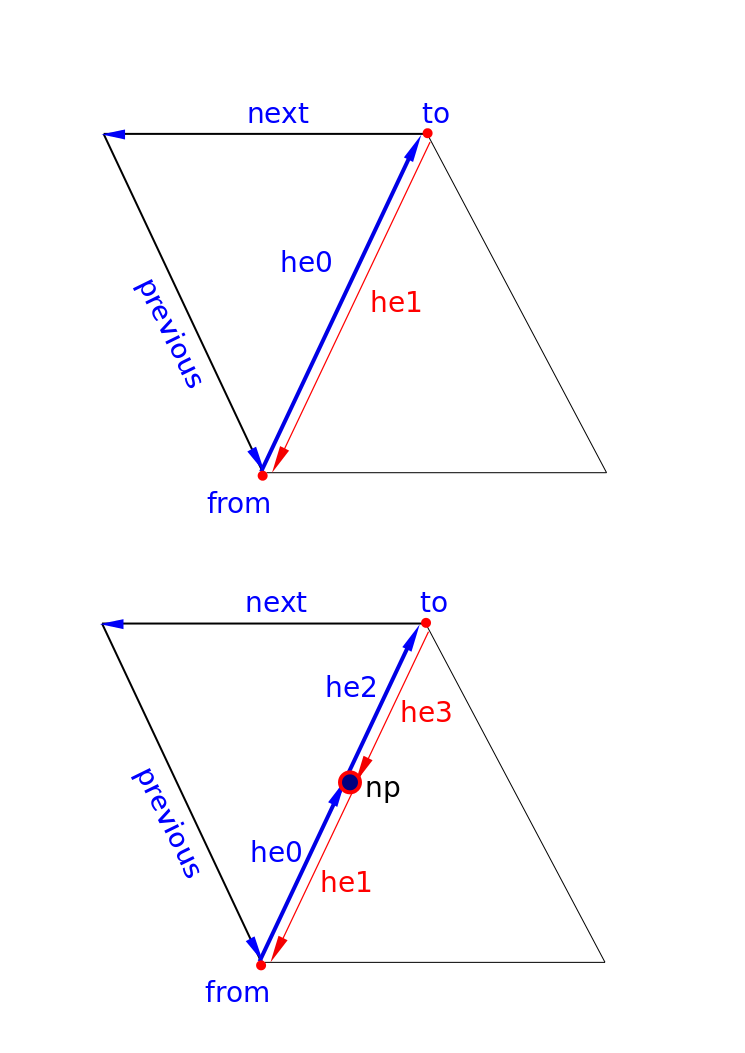
\includegraphics[width=0.8\linewidth]{figures/cutting/splitedge.png}
  \caption{\label{fig:splitedge}
  {Left: The edge to be split. Right: Splitting an edge produces a new edge from the point of 
  intersection to the original endpoint. New points $newp_0$ and $newp_1$ are initially co-located.}
}
\end{figure}


Upon topological modification, events are generated to notify cutting algorithms of the internal changes in the mesh structure. 
This is also useful for debugging and evaluation purposes and can be logged for accounting the sequence of changes made to the 
original mesh. The events include update, insertion and removal of nodes, edges, faces and elements.


In the next section we describe the cutting algorithm which is based on the edge-based data structure presented in this section.

\section{Cutting Algorithm}
\label{sec:cutalg}
Our cutting algorithm follows the same strategy presented by Ganovelli \etal \cite{Ganovelli2000} which suggests use of lookup tables to 
handle different configurations. We also applied the optimizations suggested by
Steinemann and Mor \etal \cite{Steinemann, Mor2000} to have minimal new elements added to the mesh under cut. 
The first stage in our cutting algorithm is detecting the cut sweep-surface. The input to this stage is the cut trajectory which is a list of points
that the scalpel passed through in Euclidean space. The cut trajectory is not collected until the axis-aligned bounding box of the cutting tool intersects
with that of the tissue. The tissue bounding box is expanded to rule out the boundary cases where the surface of the model contacts with its own bounding 
box. In such cases the scalpel might miss the surface if the bounding box test fails to detect the initial contact. 


\subsection{Edge Intersections}
Using a GPU kernel function the intersection of the sweep-surface and all the edges of the model are computed. 
The input to this stage is the list of edges of the model and 4 points defining the sweep-surface quadrilateral. 
Since the intersection of a triangle and a line segment is faster to compute than a quadrilateral, we 
use two intersection tests per each edge to figure out whether the segment is split or not. The implementation
of our edge triangle intersection follows the Ray-Triangle intersection test given in \cite{RTR3}.


Similar to our GPU polygonization method in section \ref{sec:surfextraction}, a prefix-sum operator counts the number
of intersections and also compacts the resulting array of intersection points. The final output of this stage is a list
of intersection points and the associated edge indices. The listing below shows the prototype of the kernel function in 
OpenCL:

\begin{lstlisting}[frame=single]
//Computes the intersection of edges and sweep surface
float sweepSurfEdgeIntersections(unsigned int countEdges,
			         __global float4* edgeBuffer,
				 __global float4 sweepSurface[4],
				 __global float4* scanIntersections,
				 __global unsigned int* scanIndices,
				 __global unsigned int* scanFlags);
\end{lstlisting}
		     
\begin{algorithm}[H]
\caption{\textit{EdgeIntersections} The kernel function that computes intersections of edges 
and the sweep-surface. The prototype of the kernel follows the listing above and the algorithm here represents one 
thread of the execution. }
\label{alg:edgeIntersections}
\begin{algorithmic}[1]	
  \IF{$dim.x \geq countEdges$}
  \STATE return
  \ENDIF
  \STATE $scanFlags[dim.x] \gets 0$
  \STATE $tri0 \gets triangle(0, 1, 2, sweepSurface)$
  \STATE $tri1 \gets triangle(0, 2, 3, sweepSurface)$
  \STATE $edge0 \gets edgeBuffer[dim.x * 2]$
  \STATE $edge1 \gets edgeBuffer[dim.x * 2 + 1]$
  \STATE $res \gets IntersectSegmentTri(edge0, edge1, tri0, p)$
  \IF{$res = 0$}
  \STATE $res = IntersectSegmentTri(edge0, edge1, tri1, p)$
  \ENDIF
  \IF{$res \neq 0$}
  \STATE $scanIntersections[dim.x] \gets p$
  \STATE $scanIndices[dim.x] \gets dim.x$
  \STATE $scanFlags[dim.x] \gets 1$
  \ENDIF
  
\end{algorithmic}
\end{algorithm}

Each thread of execution will examine one edge of the mesh. The blade quadrilateral is divided to two triangles named $tri0$ and $tri1$ 
as shown in algorithm \ref{alg:edgeIntersections}. The two endpoints of the current edge are retrieved from the mesh storage buffer called 
$edgebuffer$. The function named ``IntersectSegmentTri'' computes the intersection point of a line segment and a triangle. If the
first triangle does not intersect with the blade end-points the test is repeated for the second triangle. If there is a
valid intersection point, it is stored in the appropriate output buffer ``scanIntersections'', the index of the intersected edge is stored at
``scanIndices'' and a flag that later identifies successful intersection tests is written to ``scanFlags''. These buffers are compacted later 
using sum-scan operators discussed in the previous chapter. 


\subsection{Produce cut-node list}
Following the improvement made by Steinmann \etal \cite{Steinemann} to minimize the number of subdivided elements; 
per each intersection point which is ``too close'' to one of the edge endpoints; 
the sweep surface is snapped to that endpoint (see figure \ref{fig:cutnode}). The associated endpoint is also stored in a separate list called ``cut-nodes''. 
In our system if an intersection point lies within the 20 percent of its associated edge length radius then it is considered 
as a ``cut node''. This value avoided the most skinny elements. An analysis on the quality factors of the tetrahedral elements 
is made later in this chapter. The cut-nodes are later used to produce special subdivision cases which output non-skinny 
tetrahedral elements.

\begin{figure}[H]
  \centering
  % the following command controls the width of the embedded PS file
  % (relative to the width of the current column)
  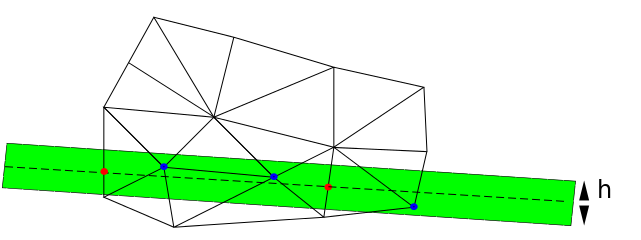
\includegraphics[width=0.8\linewidth]{figures/cutting/cutnode.png}
  \caption{\label{fig:cutnode}
  {Dashed line represents the cut trajectory. For all the edges intersected by the cut sweep surface the end point closest to the sweep surface is selected.
  If the node lies within a threshold h, it is marked as a cut-node painted in blue and all the incident edges to that node are removed from the cut-edges list.
  The red dots are the intersection points associated with the remaining cut-edges.}
}
\end{figure}

\begin{algorithm}[H]
\caption{\textit{ProduceCutNodeList} The function that builds the cut-nodes list from the intersected edges.
If an intersection is within the predefined distance of an edge endpoint it is considered as a ``cut-node''.}
\label{alg:produceCutNodes}
\begin{algorithmic}[1]	
  \FOR{$i = 0$ \TO $cutEdges.count - 1$} 
  \STATE $ce \gets cutEdges\left[i\right]$
  \STATE $edge \gets mesh.edge(ce.handle)$
  \STATE $normalizedT \gets ce.t / length(edge.from, edge.to)$
  \IF{$normalizedT < h$}
  \STATE $cutNodes.insert(edge.from)$
  \ELSE
    \IF{$normalizedT > 1.0 - h$}
    \STATE $cutNodes.insert(edge.to)$
    \ENDIF
  \ENDIF
  \ENDFOR
\end{algorithmic}
\end{algorithm}

In algorithm (\ref{alg:produceCutNodes}) the intersection distance is normalized using the length of the associated edge.
If the normalized distance is within the predefined threshold $h$ then the start point of the edge is a cutnode. Otherwise
if the condition is true on the other end point then that end point is added as the cut-node.

\subsection{Filter intersected-edges}
All the edges that are incident to a ``cut-node'' are removed from the list of intersected-edges. Since our mesh data structure 
already has the bottom-up links, it is trivial to access all the incident edges per each node. 


\subsection{Compute configuration codes for cut elements}
\label{sec:cutconfigs}
After building the list of cut-edges and cut-nodes, all the tetrahedral cells are inspected for intersection. 
The list of cut-edges and cut-nodes are implemented as hash-tables in our system, therefore, performing a query operation can be done 
in constant time and this step is not bottleneck in our system. Per each cell all the 6 edges are checked against the cut-edges hash table 
in the same order given in figure \ref{fig:tetconfig3}. If an edge is included in the cut-edges hash table then a flag bit is set for that
particular edge. The same process is performed for the 4 nodes of each cell and a 4 bits cutnode code is computed for that cell.
Using the lookup table given in table \ref{table:allcutconfigs} and the number of cut-edges and cut-nodes; per each cell a cut configuration
is computed.  If the number of cut-edges and cut-nodes are both zero then that cell is left intact otherwise it is added to the list of intersected cells
to be processed later.

\begin{table}[H]
\begin{center}
\caption{\label{table:allcutconfigs}{The following look-up table is used to differentiate between different cutting configurations based on
the number of cut-edges and cut-nodes. All cases subdivide tetrahedral elements into smaller cells except for case Z where the original
cell is left intact.}}
  \begin{tabular}{ | l | c | c | c | }
    \hline    
    type & state & \#cut edges & \#cut nodes \\ \hline \hline    
    A & complete & 3 & 0 \\ \hline
    B & complete & 4 & 0 \\ \hline
    C & progressive & 1 & 0 \\ \hline
    D & progressive & 2 & 0 \\ \hline
    E & progressive & 3 & 0 \\ \hline
    X & complete & 2 & 1 \\ \hline
    Y & complete & 1 & 2 \\ \hline
    Z & complete & 0 & 3 \\ \hline
    \hline
  \end{tabular}
\end{center}
\end{table}

Based on its cut configuration a tetrahedral cell is subdivided into smaller elements. In our system a separate lookup table is 
implemented per each of the above cut configurations. The reason is that each configuration leads to a different number of subdivided elements, however;
it is also possible to combine all lookup tables into one. Table \ref{table:lutcutA} shows the generated cells for the cut type A.
In this configuration only 3 out 6 edges of a tetrahedra are cut and that should lead to $C(n, r) = C(6, 3) = 20$ different cut edges (without repetition and
order does not matter). However, valid cut edges are the ones that separate one node from the other three that will lead to the compact lookup table in \ref{table:lutcutA}.
The first column is the cut-edge code associated with that configuration row e.g. A56 denotes cut type A with edges 3, 4, 5 being cut where each each represent one bit in 
the code. The second column is the list of generated tetrahedral cells. Cut A produces 4 cells. Nodes 0-3 are the original nodes creating the original cell. When each edge 
shown in figure \ref{fig:tetconfig3} is cut in the middle two additional nodes are added to that cell these extra nodes are defined at indices 4-15 as shown in figure 
\ref{fig:midpoints}.

The lookup table for type B is shown in table \ref{table:lutcutB}. Four edges are being cut in configuration type B and per each cell 6 sub-elements are generated.
Cutting 4 out of 6 edges should result in $C(n, r) = C(6, 4) = 15$ distinct cut-edges. However, using the same analogy only 3 valid cuts are able to split the cell 
in two disjoint parts. Those cuts are summarized in table \ref{table:lutcutB}. 

Case Z is trivial since the cell is left intact. For case Y two tetrahedral elements are being generated and one edge is being split only. Case X is very similar to
A in the sense that one original node is being separated from the rest of the simplex. In cases X and Y the cut-nodes are duplicated and the new cells are generated based
on the split edges and the original nodes and their associated duplicates. Since we haven't implemented progressive cutting yet cases C, D and E are left for the future work.

\begin{table}[H]
\begin{center}
\caption{\label{table:lutcutA}{Lookup table for generating sub-elements for type A configuration}}
  \begin{tabular}{ | l | c | c | }
    \hline    
    config & cut edges & generated cells \\ \hline \hline    
    A56 & 3, 4, 5 & \{0, 12, 10, 14\}, \{3, 13, 11, 15\}, \{3, 1, 15, 11\}, \{1, 2, 3, 11\} \\ \hline
    A37 & 0, 2, 5 & \{1, 4, 8, 15\}, \{3, 9, 5, 14\}, \{0, 3, 14, 5\}, \{0, 2, 3, 5\} \\ \hline
    A11 & 0, 1, 3 & \{2, 5, 6, 11\}, \{3, 7, 10, 4\}, \{3, 1, 4, 10\}, \{0, 1, 3, 10\} \\ \hline
    A22 & 1, 2, 4 & \{3, 13, 9, 7\}, \{1, 8, 12, 6\}, \{1, 2, 12, 6\}, \{0, 1, 2, 12\} \\ \hline
    \hline
  \end{tabular}
\end{center}
\end{table}

\begin{table}[H]
\begin{center}
\caption{\label{table:lutcutB}{Lookup table for generating sub-elements for type B configuration. 
Sub-elements are separated by semi-colon to fit on the line.}}
  \begin{tabular}{ | l | c | c | }
    \hline    
    config & cut edges & generated cells \\ \hline \hline    
    B46 & 1, 2, 3, 5 & \{2, 6, 11, 1; 8, 11, 15, 1; 6, 11, 8, 1; 3, 7, 9, 10; 3, 10, 0, 9; 0, 14, 10, 9\} \\ \hline
    B51 & 0, 1, 4, 5 & \{3, 7, 13, 15; 15, 1, 4, 7; 15, 1, 3, 7; 0, 12, 14, 6; 2, 5, 6, 14; 0, 14, 6, 2\} \\ \hline
    B29 & 0, 2, 3, 4 & \{4, 10, 12, 0; 0, 8, 12, 4; 0, 8, 1, 4; 3, 9, 13, 5; 2, 5, 11, 3; 3, 13, 5, 11\} \\ \hline
    \hline
  \end{tabular}
\end{center}
\end{table}



\begin{figure}[H]
  \centering
  % the following command controls the width of the embedded PS file
  % (relative to the width of the current column)
  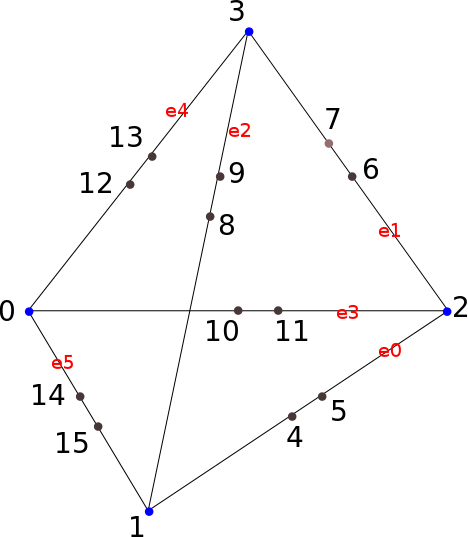
\includegraphics[width=0.4\linewidth]{figures/cutting/midpoints.png}
  \caption{\label{fig:midpoints}
  {Nodes 0-3 are the original cell nodes shown in blue dots. Splitting each of the 6 edges can produce two additional nodes up to 12 more nodes which 
  are placed at indices 4-15 shown in black dots.}
}
\end{figure}
%The main contribution of our cutting method is the GPU-accelerations applied to the cutting process to support interactive topological 
%modifications and the post processing step that supports smoothness of the cuts in case of complex tissues. 

\subsection{Topological Updates}
During the cutting process, the intersected cells are being replaced by sub-cells as discussed in the previous section. Cell removal operation involves updating the entire 
mesh structure which can be expensive if performed during the cut process. In our system all the intersected cells are being placed on a pending list for later deletion 
which will be visited by a post-processing stage called ``garbage collection''. This way the indices of the mesh entities are left intact during the cutting process and 
then once the cut is finalized the mesh can be cleaned and any unused entities such as cells, faces, edges or nodes are being purged to keep the structure as compact as 
possible for the next cutting operations.

\section{Cutting Results}
\label{sec:cutres}
In this section we review the results for the cutting algorithm presented in this chapter. 
Two models are considered for this analysis and a more complex cutting scenario is presented in chapter \ref{chapter:evaluation}.
The model shown in figure \ref{fig:dumbelsexample} is composed of two implicit spheres that are blended and tetrahedralized for 
physics simulation. The resulting volumetric mesh is cut horizontally, vertically and diagonally using the scalpel tool. 

\begin{figure}[H]
  \centering
  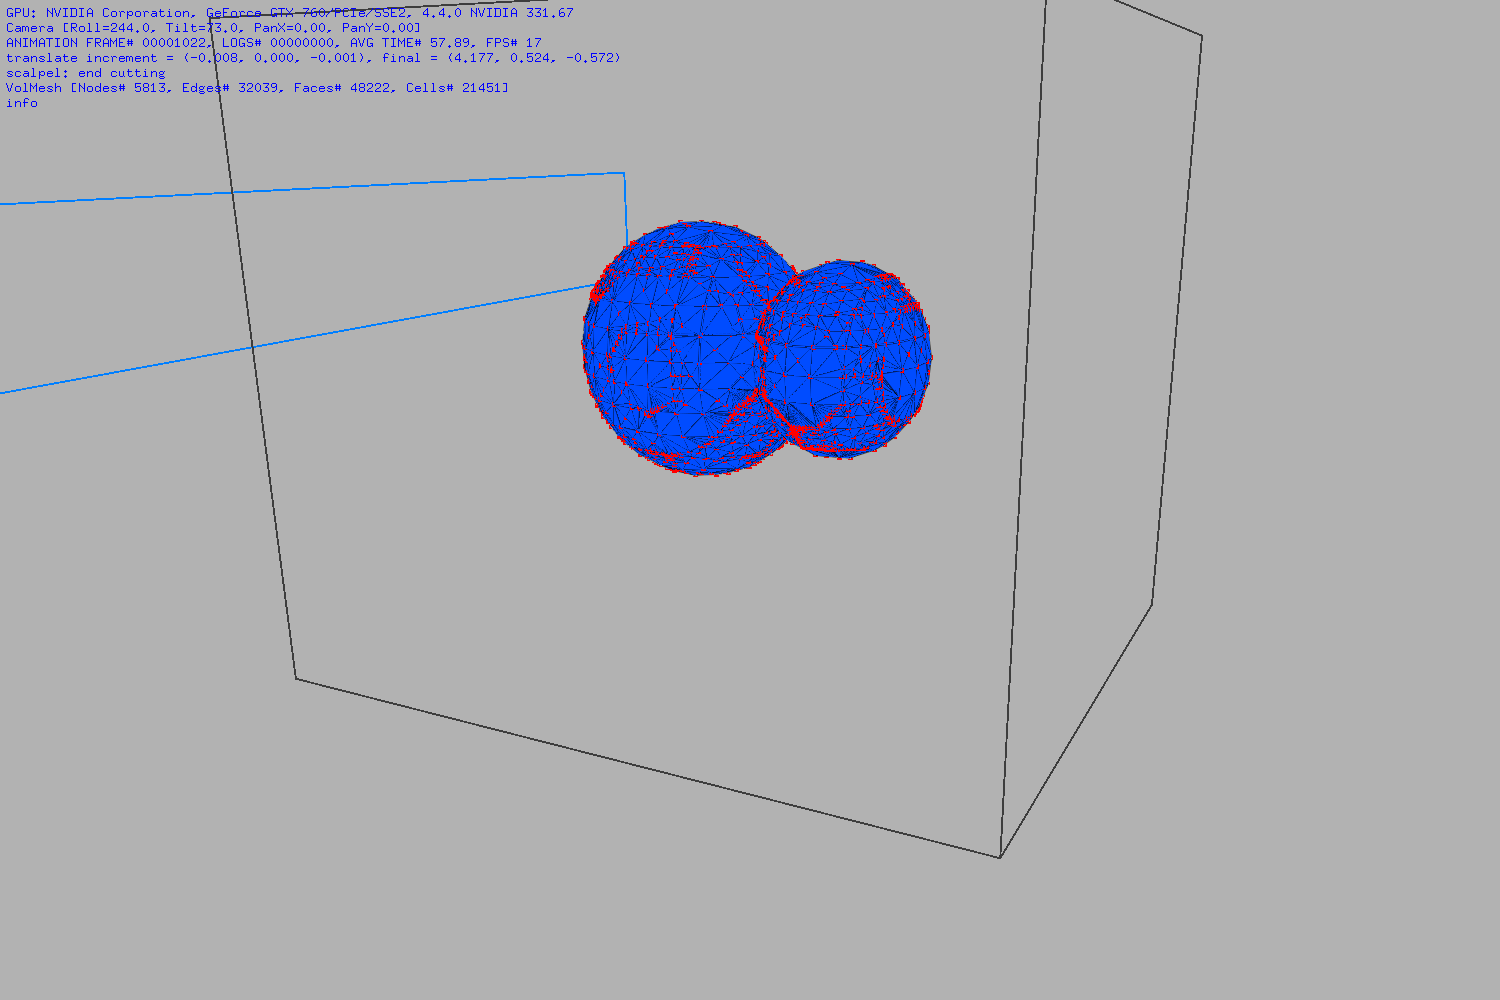
\includegraphics[width=0.4\linewidth]{figures/cutting/dumbel01.png}
  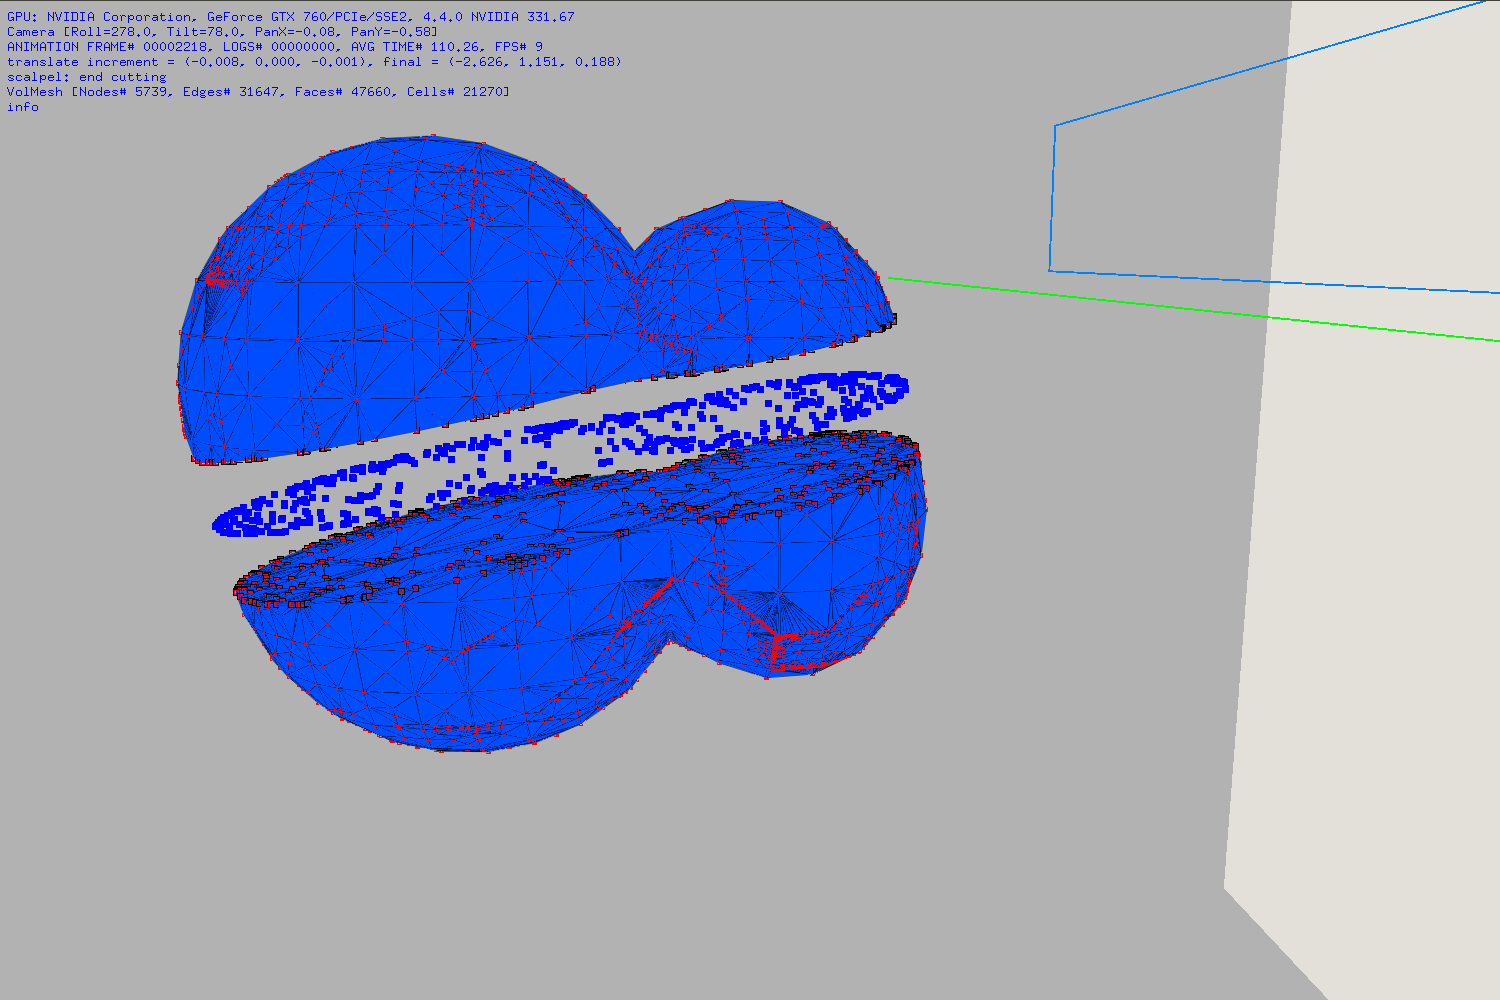
\includegraphics[width=0.4\linewidth]{figures/cutting/dumbel02.png}
  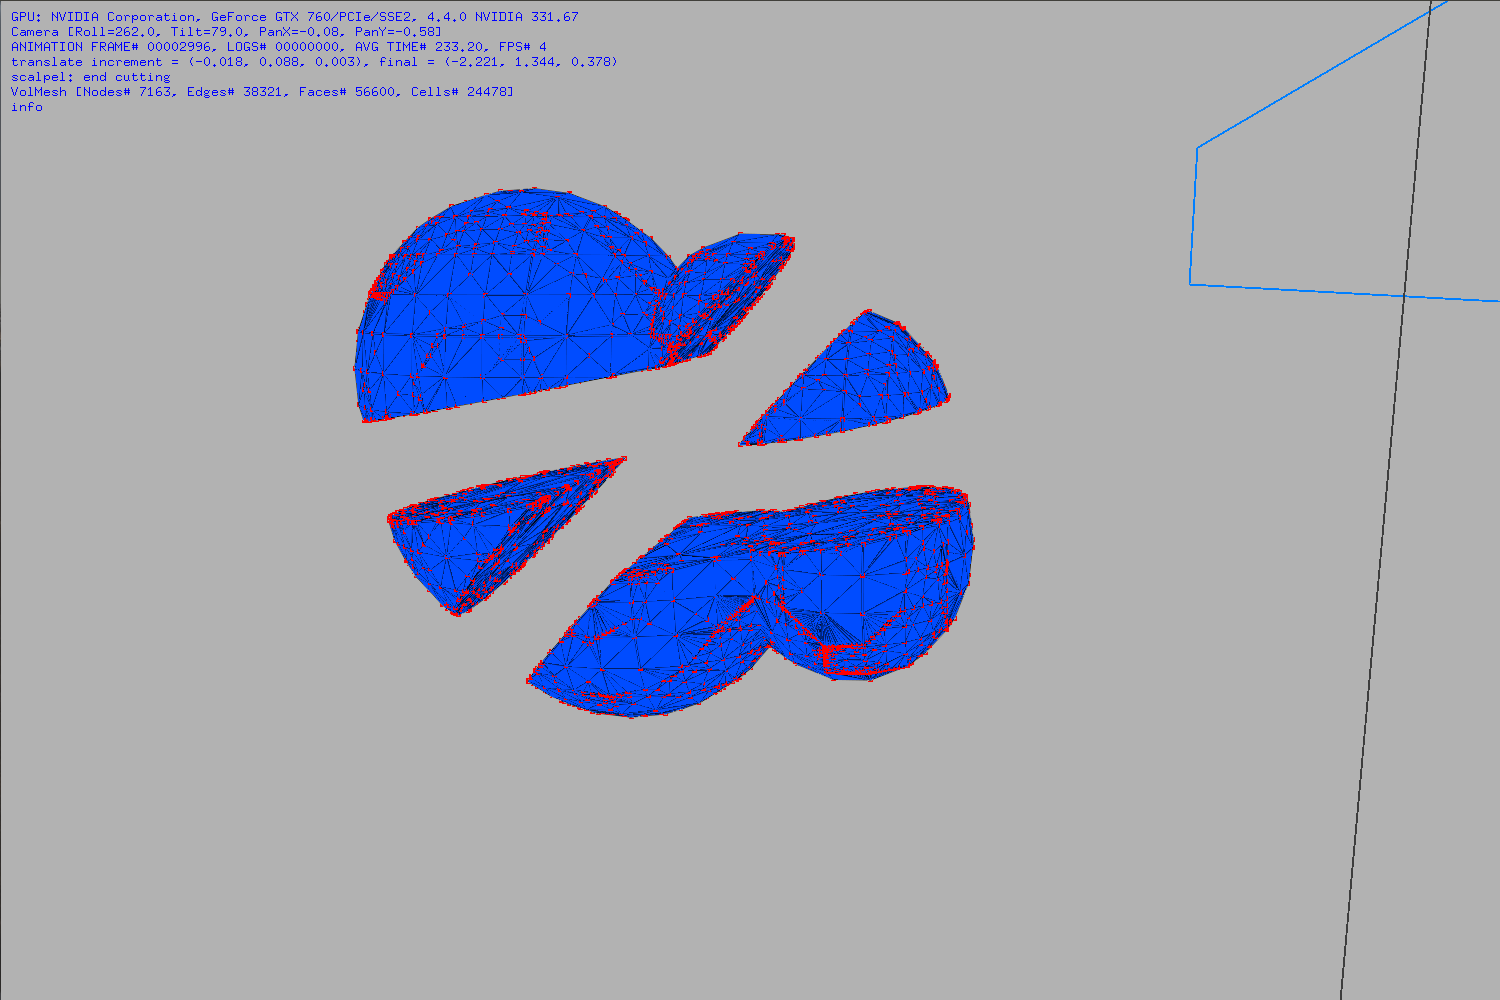
\includegraphics[width=0.4\linewidth]{figures/cutting/dumbel03.png}
  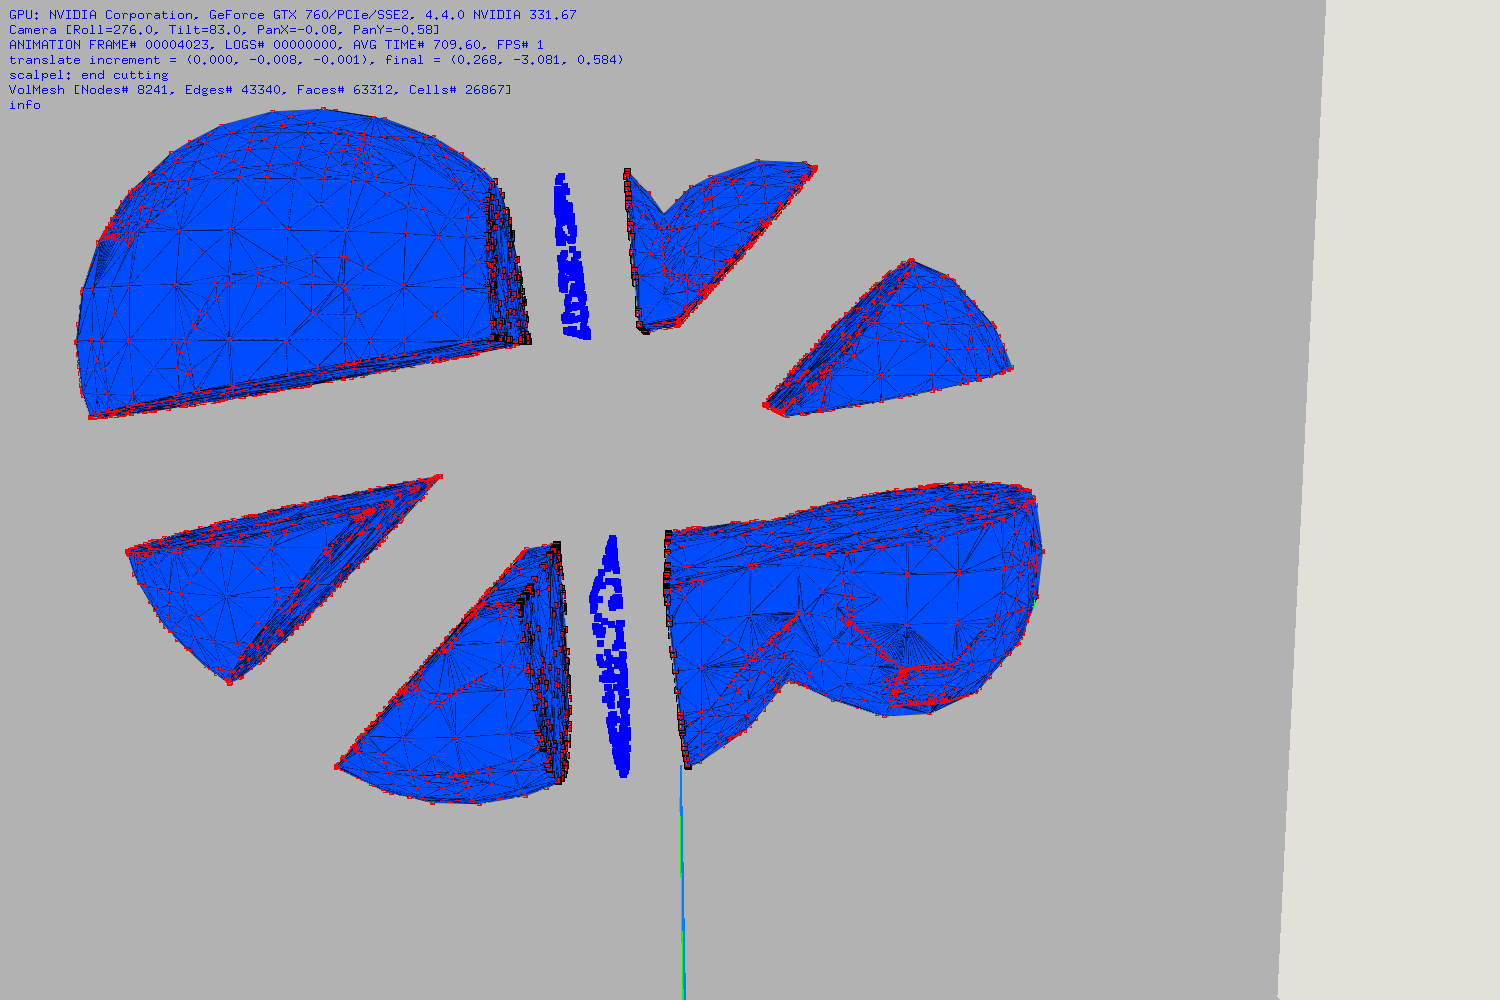
\includegraphics[width=0.4\linewidth]{figures/cutting/dumbel04.png}
  
  \caption{\label{fig:dumbelsexample}
  {Two implicit spheres are blended and tetrahedralized for our physics simulation system. The peanut model is cut 3 times.
  Top-Left: The original volumetric mesh. Top-Right: Model cut horizontally with the scalpel tool.
  Bottom-Left: Diagonal cutting, Bottom-Right: Vertical cut. Blue dot represent the intersection points on the original edges.}
}
\end{figure}

The second model is the tumor model composed of 10 blended spheres. Using the same process the model is tetrahedralized for physical simulation
and cut 3 times. Figure \ref{fig:tumor} shows the result of these topological modifications.


\begin{figure}[H]
  \centering
  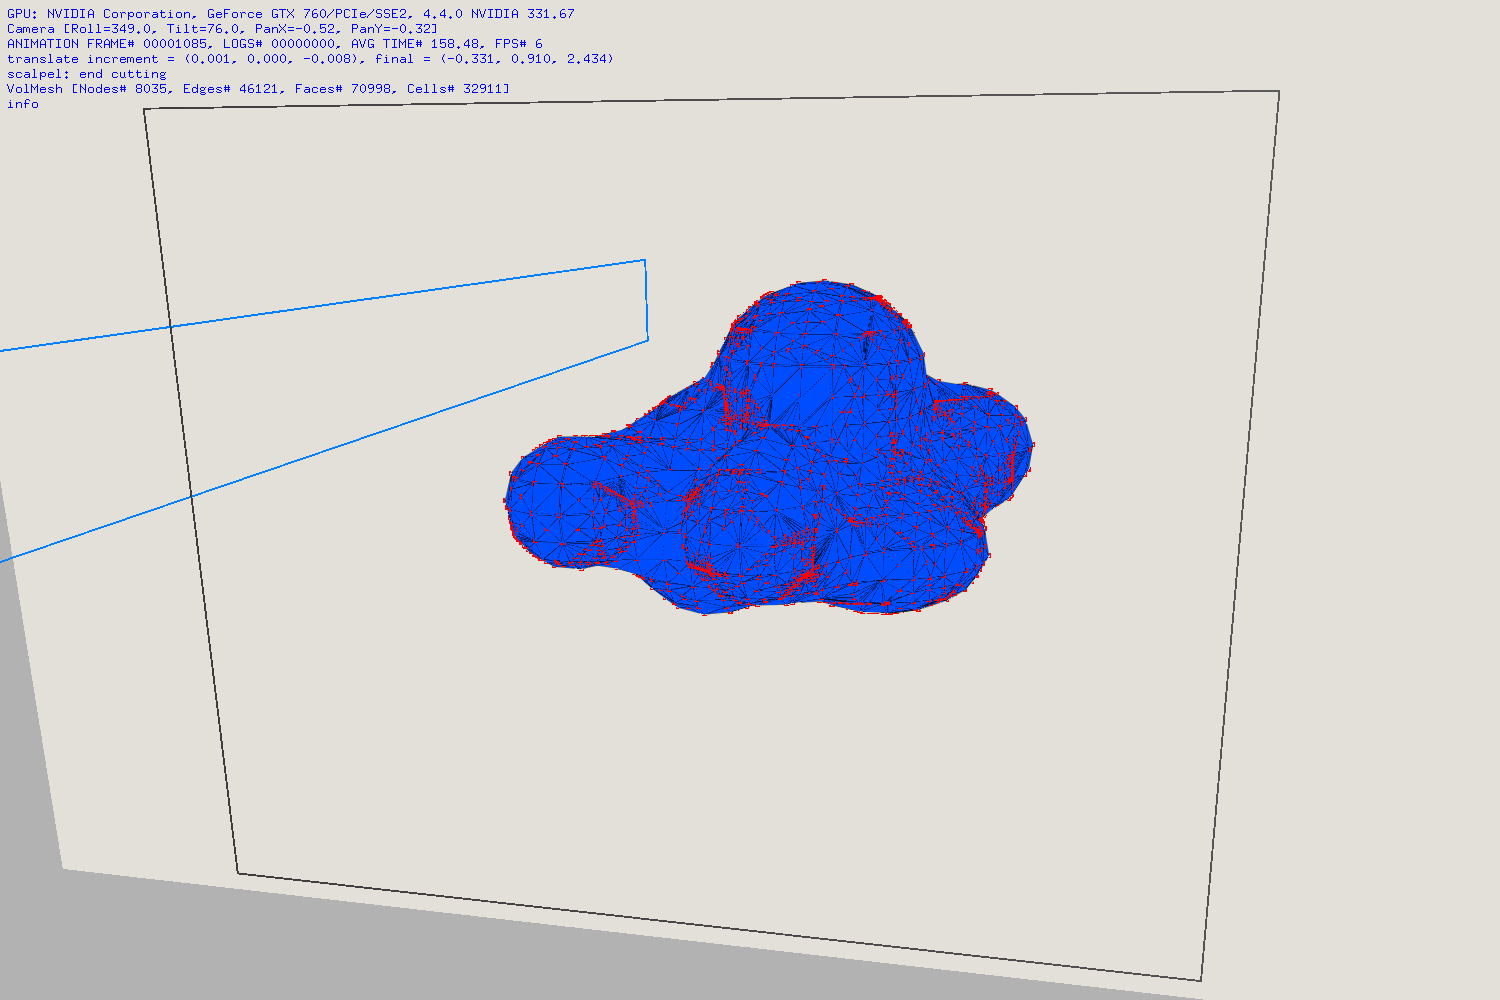
\includegraphics[width=0.4\linewidth]{figures/cutting/tumor01.png}
  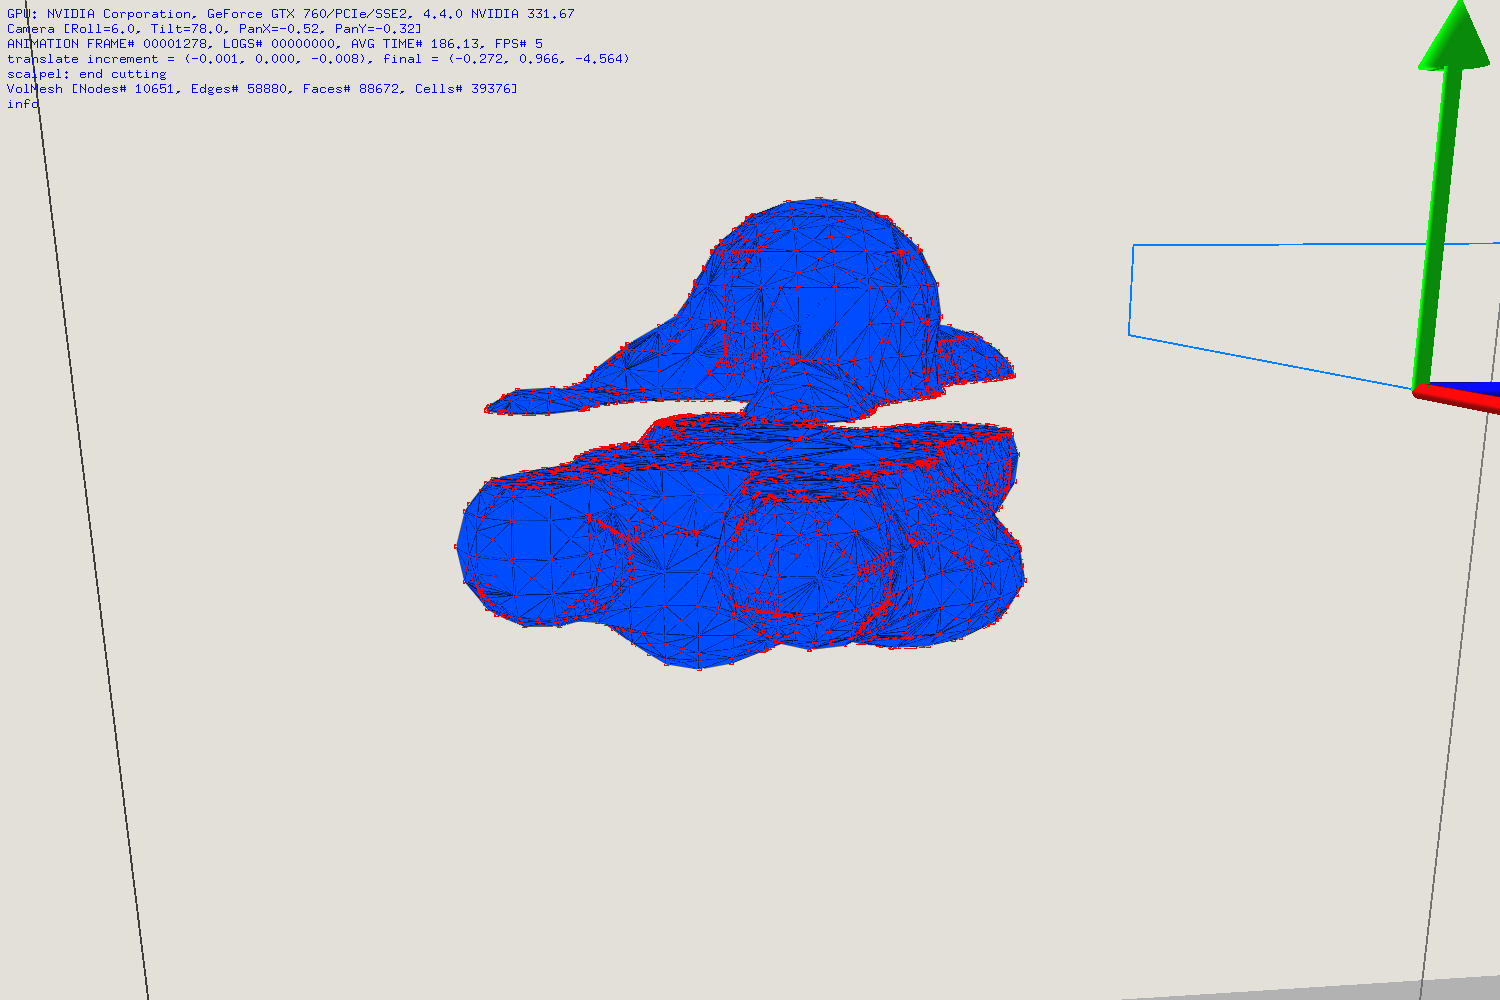
\includegraphics[width=0.4\linewidth]{figures/cutting/tumor02.png}
  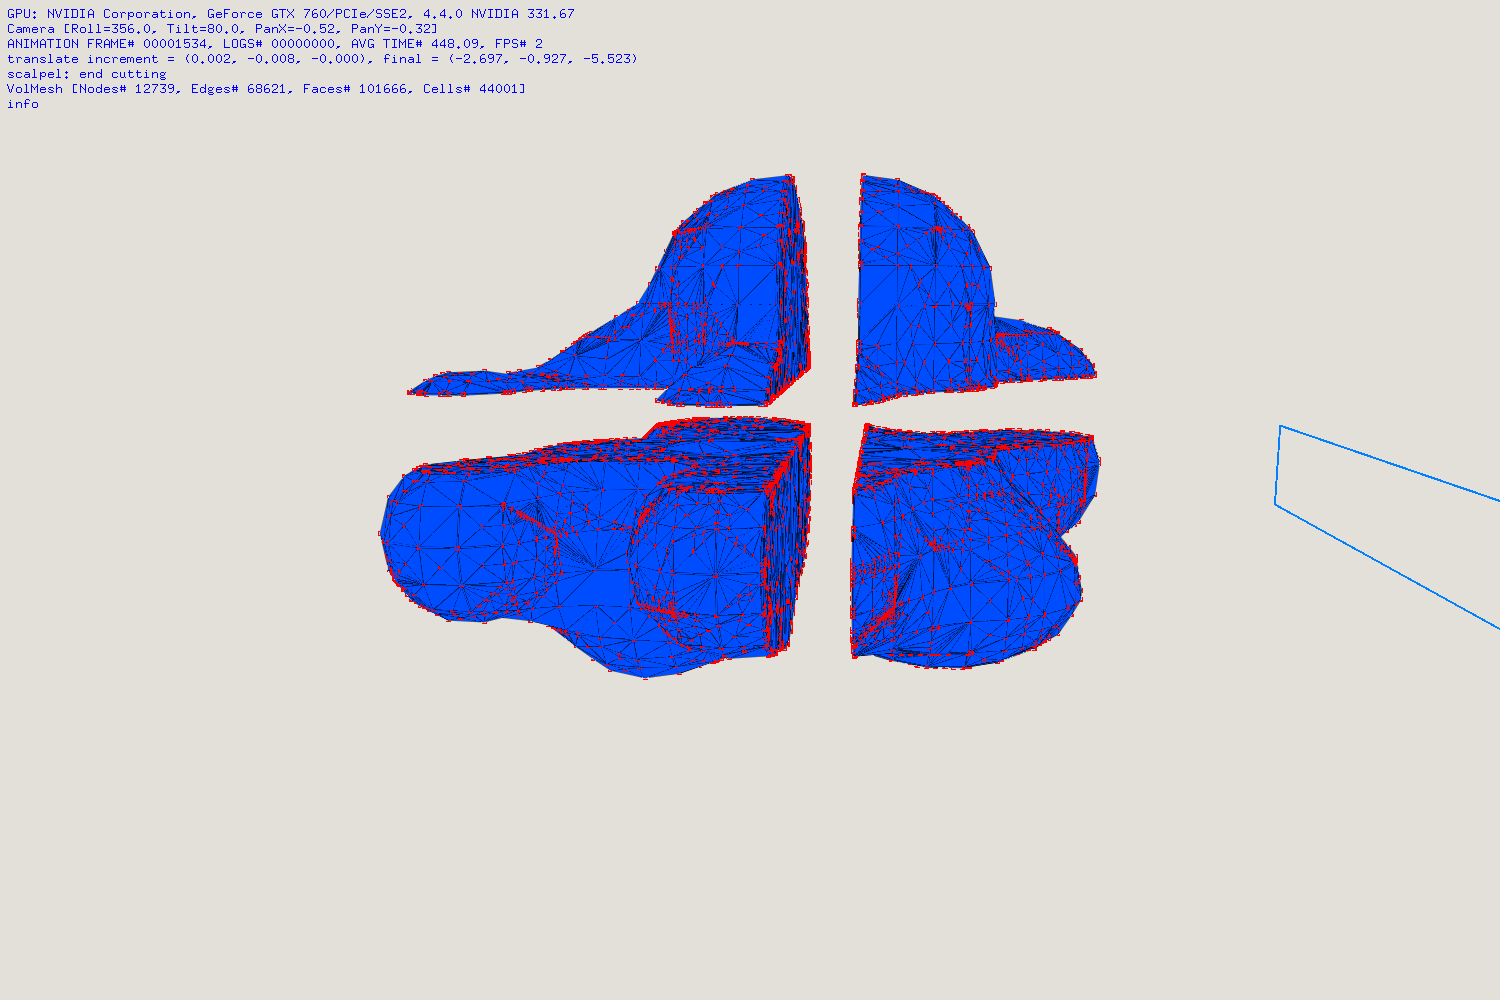
\includegraphics[width=0.4\linewidth]{figures/cutting/tumor03.png}
  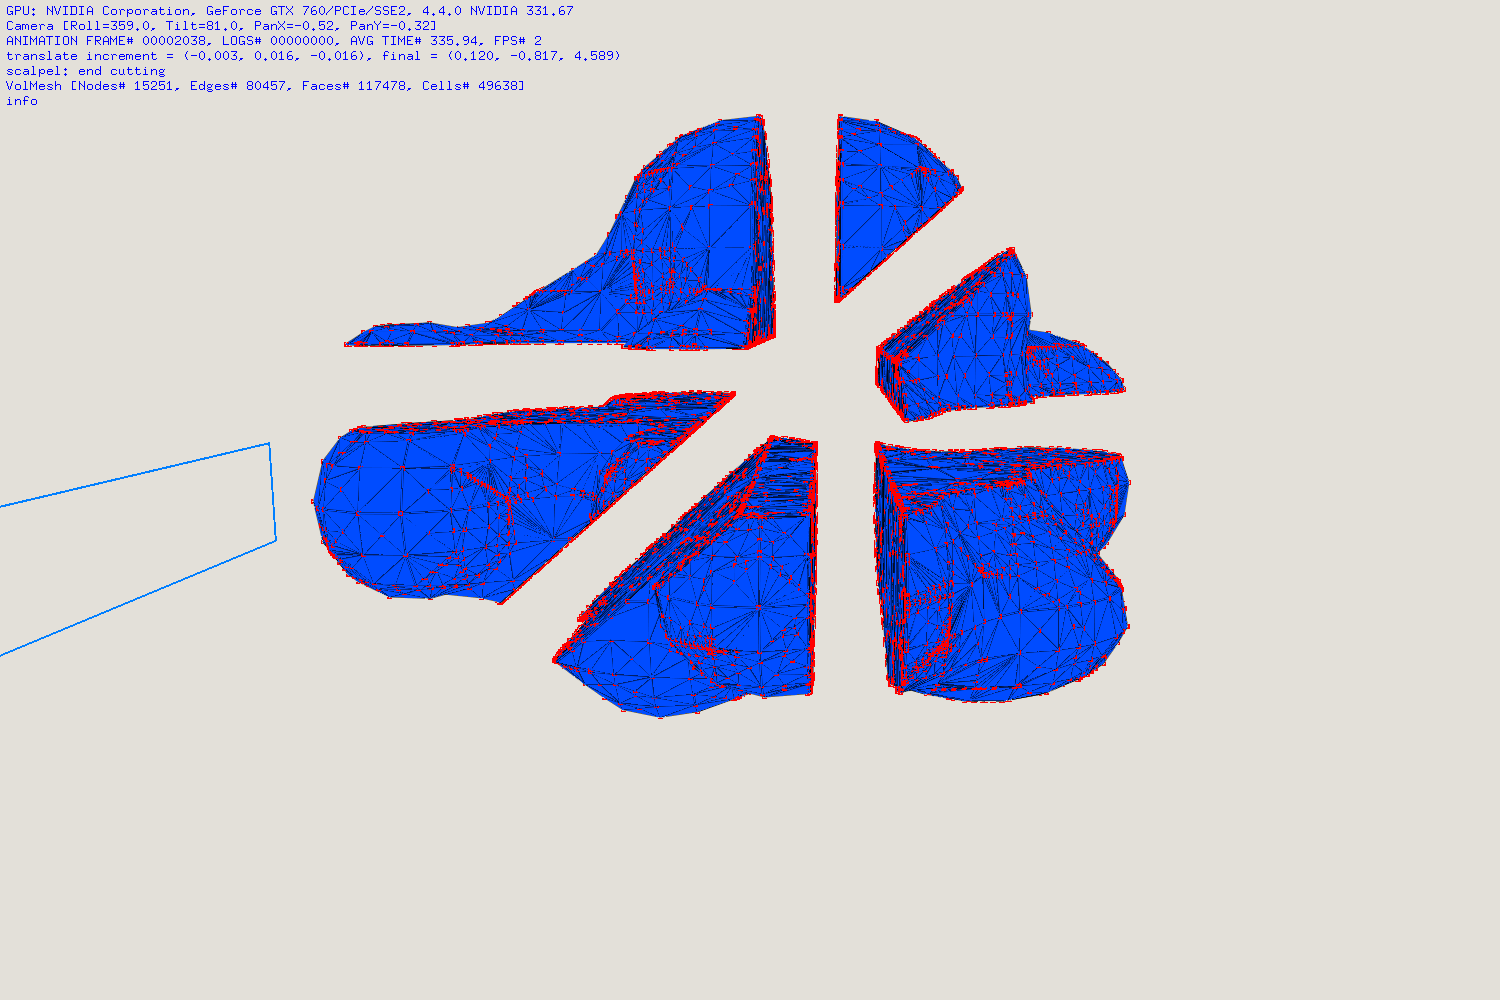
\includegraphics[width=0.4\linewidth]{figures/cutting/tumor04.png}
  
  \caption{\label{fig:tumor}
  {The tumor model above is composed of 10 point primitives and a blending operator. Top-Left: the original mesh, Top-Right:
  The mesh after a horizontal cut, Bottom-Left: The vertical cut, Bottom-Right: mesh after a diagonal cut.}
}
\end{figure}

To analyse the quality of the tetrahedral mesh after the cutting process several attributes are being considered. First, the 
number of elements before and after each cut. More elements will increase the system solve time and degrade the performance of the 
physical simulation due to the larger matrix dimensions involved in the process. Badly shaped (skinny) tetrahedral elements impose stricter constraints 
on the simulation time step \cite{Steinemann, Ganovelli2000}. In order to get an understanding of the quality of the tetrahedral mesh after the cuts, element
counts and several other quality measures are considered \cite{parthasarathy1994comparison}. 

\begin{itemize}
 \item The ratio between largest and smallest tetrahedron volume
 \item The ratio between largest and smallest edge length
 \item The lowest aspect ratio of all tetrahedra 
\end{itemize}

The aspect ratio of a tetrahedra is measured as following:

\begin{equation}
\beta = \frac{CR}{3*IR} 
\end{equation}

Where $CR$ is the circumsphere radius of an element and $IR$ is the inscribed-sphere computed by the following equation 
\cite{parthasarathy1994comparison}:

\begin{equation}
IR = \frac{4V}{\sum_{i=1}^{4} SA_i}
\end{equation}

Where $V$ is the volume of a tetrahedra, $SA_i$ is the surface area of the $i$th triangle face of an element.
 
\begin{table}[H]
\begin{center}
\caption{\label{table:meshquality}{Mesh quality measurements.}}
  \begin{tabular}{ | l | c | c || c | c |}
    \hline    
     & original peanut & peanut after 3 cuts & original tumor & tumor after 3 cuts \\ \hline \hline    
    Nodes & 4437 & 8933 & 8035 & 15821  \\ \hline
    Edges & 25420 & 46466 & 46121 & 82711 \\ \hline
    Faces & 39108 & 67388 & 70998 & 120212 \\ \hline
    Cells & 18124 & 28322 & 32911 & 50605 \\ \hline
    $V_{max} / V_{min}$ & 84.927 & 58.253 & 316.898 & 287.596 \\ \hline
    $l_{max} / l_{min}$ & 42.367 & 47.547 & 40.045 & 130.556 \\ \hline
    $AspectRatio_{min}$ & $3 \times 10^{-7}$ & $3 \times 10^{-7}$ & $10^{-6}$ & $10^{-6}$ \\ \hline
    \hline
  \end{tabular}
\end{center}
\end{table}

Graichen \etal presented an excellent study on the tetrahedral mesh quality measures \cite{Graichen1993}. 
Thin, wedge-like, flat and sliver elements (where 4 points of the element are co-planar) are the source of poor simulation 
results. Table \ref{table:meshquality} summarizes the statistical quality factors before and after cutting the two example meshes. 
The original volumetric mesh of both of these models are extracted from their associated \blob representation using our GPU tetrahedralization
algorithm presented in chapter \ref{chapter:GPUDiscretization}.

As it can be seen from the results the cutting method presented in this chapter does not increase the ratio of maximum to minimum 
volume after the cuts are being made. This means that the element subdivision stage in our system does not 
introduce ill-shaped elements to the mesh. The ratio of the maximum to minimum edge-length did not change drastically.
However, a local re-meshing process after the cut specially in the vicinity of the cut region can improve the quality 
of the mesh significantly. 

The element count has increased steadily after each cut operation. Figure \ref{fig:cutting_cells_increase} shows the trend of element increase 
after $N$ cuts are made to the mesh.

\begin{figure}[H]
  \centering
  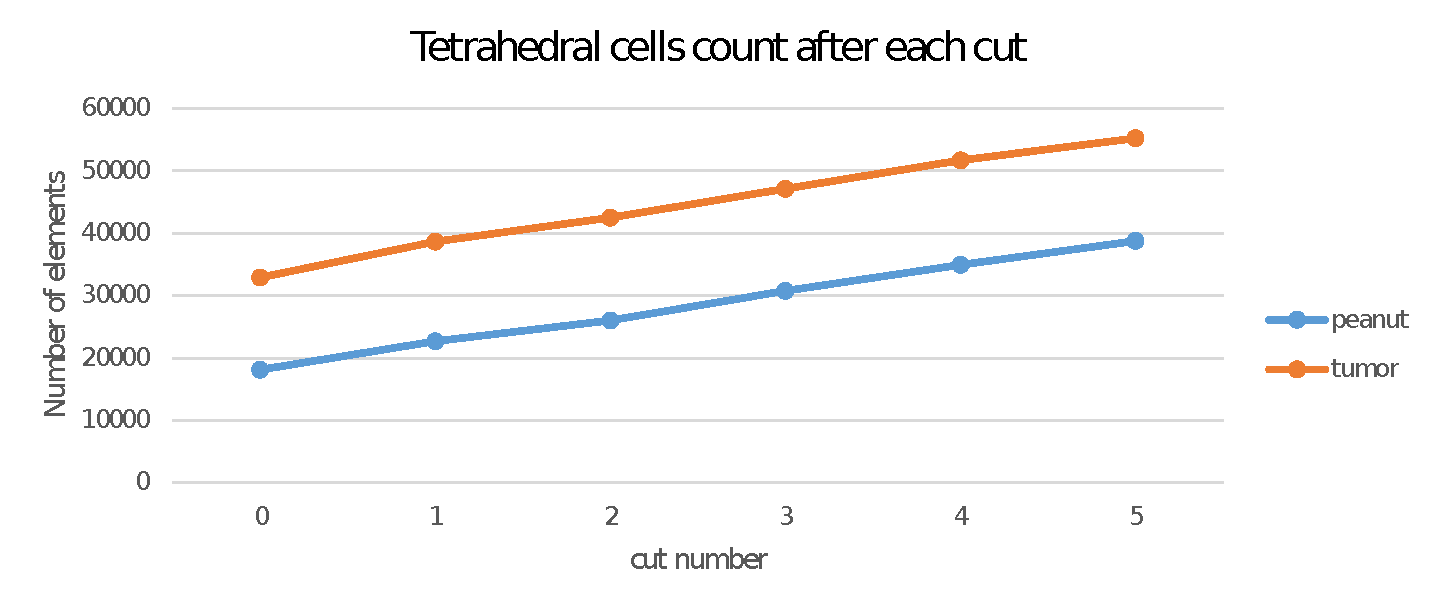
\includegraphics[width=1.0\linewidth]{figures/cutting/cutting_cells_increase.pdf}
  \caption{\label{fig:cutting_cells_increase}
  {Number of tetrahedral cells after each cut operation. The horizontal axis is the cut number starting from cut 0 or the original mesh. 
  The vertical axis is the number of cells.}
}
\end{figure}

Figure \ref{fig:cutting_intersected_vs_new} provides a clear understanding of how many new cells are being added to the mesh after each cut operation.
The blue bar in this figure shows the number of cells that are intersected with the cut surface per each cut. Following the algorithm given in 
section \ref{sec:cutconfigs} the intersected cells are being subdivided and replaced by new set of generated cells shown in orange. 
On average the ratio of newly generated cells to intersected cells is 3.6 from these results. This is due to the fact that most of the cut configurations
are of type A which result in a 1 to 4 subdivision. 

\begin{figure}[H]
  \centering
  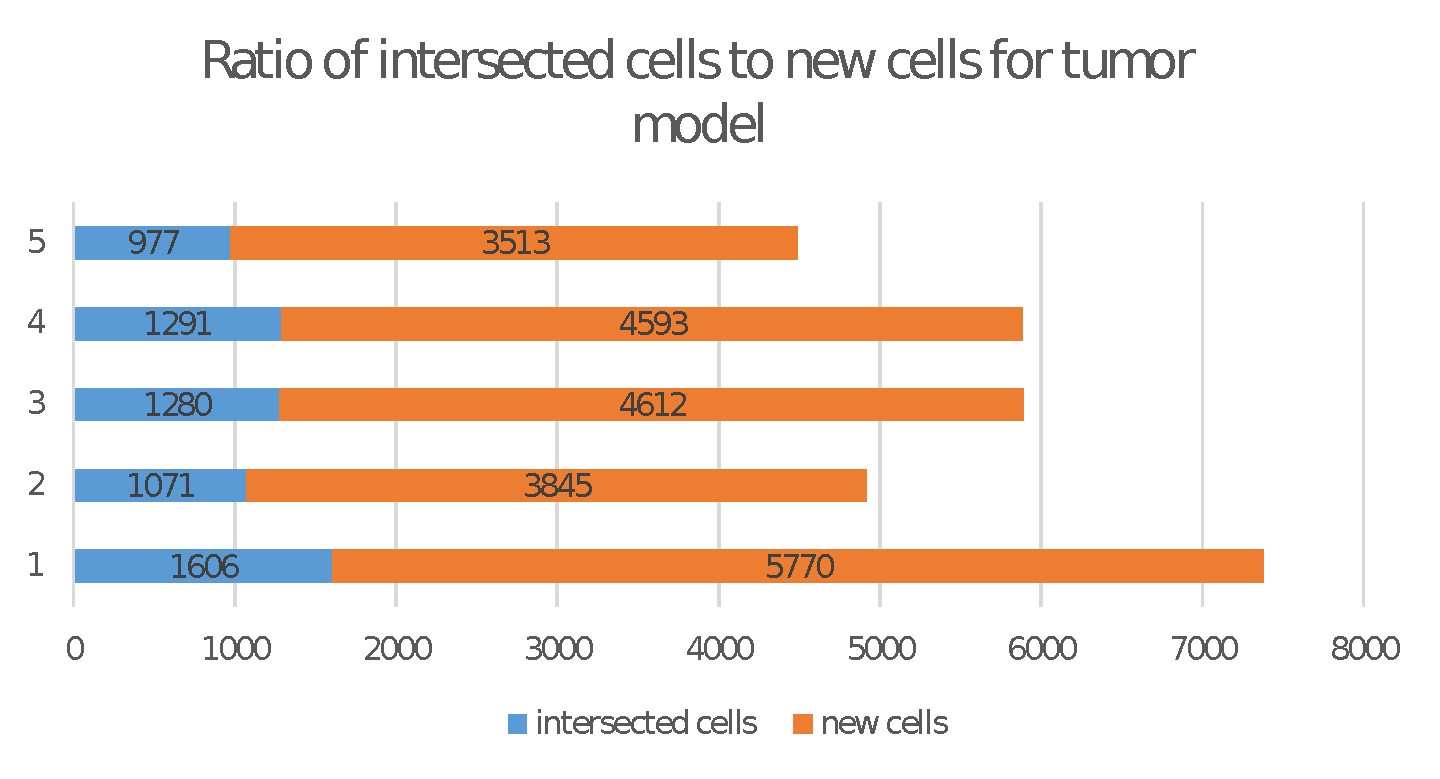
\includegraphics[width=1.0\linewidth]{figures/cutting/cutting_intersected_vs_new_tumor.pdf}
  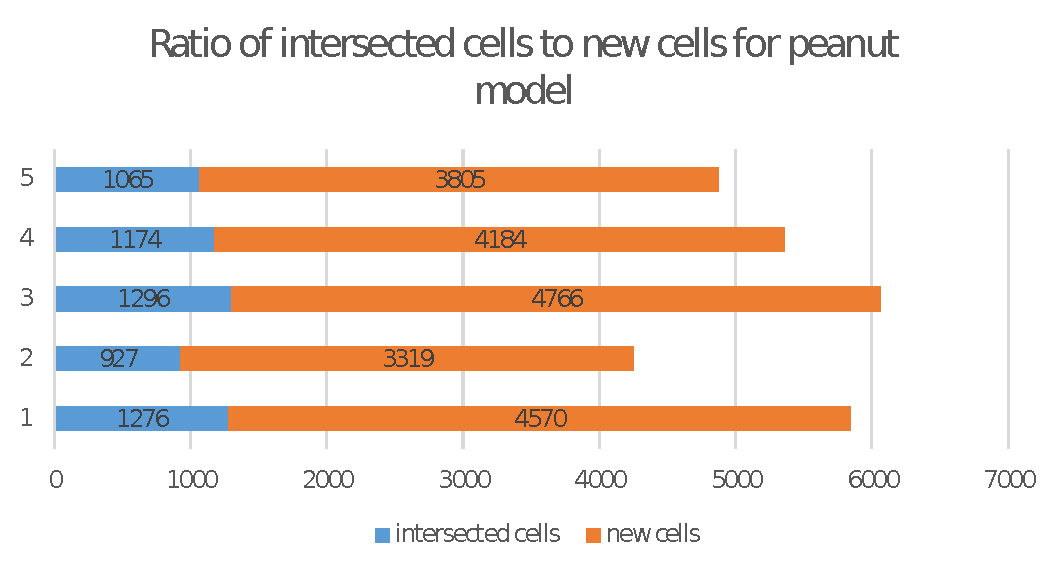
\includegraphics[width=1.0\linewidth]{figures/cutting/cutting_intersected_vs_new_peanut.pdf}
  \caption{\label{fig:cutting_intersected_vs_new}
  {The ratio of intersected cells to newly added cells for tumor (top) and peanut model (bottom). Each blue bar represents the count of cells 
  intersected with the scalpel tool while the orange bar next to it, is the number of newly generated cells after subdividing those intersected cells.}
}
\end{figure}

